\documentclass[12pt,a4paper]{article}
\usepackage{authblk}
\usepackage[margin=1in]{geometry}
\usepackage{fancyhdr}
\usepackage{hyperref}
\usepackage{graphicx}
\usepackage{babel}
\usepackage{csquotes}
\pagestyle{fancy}

\title{GPT Pedagogy}
\author[1]{Matthew Pisano\quad\href{mailto:pisanm2@rpi.edu}{pisanm2@rpi.edu}}
\author[1]{\\Tiburon Benavides\quad\href{mailto:benavt@rpi.edu}{benavt@rpi.edu}}
\author[1]{\\Lu Zhou\quad\href{mailto:zhoul12@rpi.edu}{zhoul12@rpi.edu}}
\author[1]{\\Yanshen Lin\quad\href{mailto:liny16@rpi.edu}{liny16@rpi.edu}}
\author[1]{\\Yiyang Cai\quad\href{mailto:caiy3@rpi.edu}{caiy3@rpi.edu}}
\affil[1]{Rensselaer Polytechnic Institute}
\date{\today}

\begin{document}
    \maketitle

    \abstract{
        GPT-3 is a Large Language Model that, through overuse, is often used to deprive students of the
        opportunity to learn effectively. Our intended use case of GPT enables the
        transparent use of the technology between instructor and student. We aim to create a
        more active and participatory learning environment through the usage of the model in active
        learning. Our long-term goal for higher education is along the lines of the fourth UN SDG:

        \begin{quote}
            Ensure inclusive and equitable quality education and promote lifelong
            learning opportunities for all.
        \end{quote}

        We view GPT as a way to create an adaptive learning experience which promotes the educational
        endeavor rather than detracts from it.

        Our plan is to develop a GPT-3 based learning assistant for the \textit{Introduction to Biology}
        course here at RPI.  Through a partnership with the professor, we will gather sufficient amounts
        of course material to fine-tune a pre-trained GPT-3 model. This will create a knowledgeable
        and focused learning assistant, \textit{Mathesis} (from the ancient greek work for learning).
        By creating this personalized AI tutor we can make it easier and more transparent for
        students to learn the material and reduce their stress.

        One of our goals is for the model to maintain its conversational abilities while embedding
        additional knowledge about faculty defined key learning objectives. \textit{Mathesis} will
        generate a series of topic-relevant questions, evaluate the answers of those questions, and give
        useful feedback or counter-examples to the student. The model benefits from human-in-the-loop
        reinforcement learning by storing previous chats from students and faculty alike.

        We also aim for this model to be generalizable to other classes and disciplines in the future.
        The model will work especially well for courses where it is difficult to give personalized
        feedback to each learner in each class meeting time. This often happens in classes that have
        a high student to faculty ratio. It will also work well for courses with students, interested
        in AI, who cannot adequately engage with that interest through the course material.
    }

    \pagebreak
    \section{Introduction}

    The idea for this project was conceived before the beginning of our Informatics class.
    It stemmed from observations about the direction that large language models are currently
    heading in, and how many educational institutions are not fully prepared to handle the
    fallout of this trend.  Our primary motivation for this project is to remedy this issue.  By
    providing students with an opportunity to use large language models, like GPT, as a learning tool,
    we allow students to gain valuable insight into the practical benefits and shortcomings of these models.

    \subsection{Our Targeted Approach}

    When looking at our project through a more focused lens, we believe that it will benefit the
    students in the courses that \textit{Mathesis} may be integrated into.  For many introductory
    classes, their main focus is to imbue students with a large amount of foundational
    knowledge before they explore the specifics in subsequent classes.  We believe that
    a GPT model will have a significant impact in helping with this task.  By fine-tuning a model
    on a large amount of course material, it will be able to provide relevant questions to students
    with greater detail and with a stronger relation to the other topics in the course.  This comes
    along with the large amount of general knowledge that the model initially has.  While it may
    not be able to go into detail about very niche topics, fine-tuning allows it to provide adequate
    detail on the material that students need to learn.

    \subsection{Broad Impact}

    From a broader perspective, customized learning assistants, similar to ours, have the potential
    to make a significant impact on the educational landscape as a whole.  One of the biggest issues
    that our project addresses is the asymmetric distribution of faculty time between students.
    Many courses at RPI, especially one or two thousand level courses, have a very high student to
    faculty ratio.  Due to this, each student is only afforded a very limited amount of one-on-one
    time with the professor or their TAs.  Automated learning assistants like \textit{Mathesis} can
    help to afford students more time with a knowledgeable entity in their field.  This effect would
    not only benefit students at RPI, but also nearly every other student in every other institution.
    While models such as ours cannot serve as a complete replacement for faculty, they can instead
    serve as an aide, answering students' questions and providing helpful feedback.  The more
    competent this model, the less one-on-one time students will need to spend with faculty.  This
    will hopefully result in a more complete understanding of the course material among the students.

    \subsection{Aristotle For All}

    This asymetry has served as a large motivator for us while working on this project.  The opportunity to
    both free up faculty to have more personalized time with each student and to allow each student
    to have a personal tutor by their side will help to solve many of the struggles that students
    have with learning in general.  These ideas are reflected in both past and contemporary sources.
    In a very similar vein to our project, Khan Academy's \textit{Khanmigo}~\cite{khanmigo} model
    aims to provide a very similar service to students through the internet.  Our hope is that
    \textit{Mathesis} will soon serve a similar role, but customized for RPI's students and
    curriculum.  These ideas are reflected in the well researched, and somewhat prophetic, video
    \textit{Digital Aristotle: Thoughts on the Future of Education}~\cite{aristotle} by CGP Grey.  It outlines
    many of the same points that we have mentioned here in addition to detailing how technologies
    such as \textit{Mathesis} or \textit{Khanmigo} can have on the future of education.

    \section{Project Use Case}

    \subsection{Specifications}

    For the development of the use case for this project, it is important to detail several
    specifications that describe GPT Pedagogy in a more rigorous manner.  One of these specifications
    is the list of the requirements of the project.  To fulfil our objectives, the
    project has the following \textit{functional requirements}:

    \begin{itemize}
        \label{functionalReqs}

        \item Provide students with a knowledgeable teacher that can answer any course-relevant question
        \item Be able to automatically generate a series of evaluation questions for students and
        reference answers based on the core topics of the course
        \item Receive students' answers to evaluation questions and evaluate their correctness based
        off of the reference answers
        \item Provide useful feedback to students if their answers did not sufficiently match the
        reference answers
        \item Allow instructors to review and regenerate all questions generated by the model
        \item Allow instructors to evaluate a summary of student performance based off of the
        automatically generated questions
    \end{itemize}

    Along with these functional requirements, the project requires several \textit{non-functional
    requirements}.  Our project must also have:

    \begin{itemize}
        \label{nonFunctionalReqs}
        \item A GPT model that can respond in a conversational and contextually sensitive manner
        \item That model be fine-tuned on relevant course material to narrow its focus of expertise
        \item A front end environment that allows students and administrators to interact with the model
        \item A login and authentication system to prevent unwanted access and to keep track of evaluations
    \end{itemize}

    Another important specification to consider is that of the entropy/uncertainty of the project.
    Overall, we have worked to minimize the total uncertainty of the project.  It is important to note,
    however, that the GPT model will always introduce some amount of extra uncertainty.

    One of the areas where we worked to minimize the uncertainty in was the user interface.  This is
    split into two parts, the student and administrator views.  In both of these cases, our design
    was oriented towards a simple, straightforward interface.  We worked to accomplish this through
    the use of a minimalist design.  Users can choose to choose only a few tabs: the main chat and
    the lesson evaluations.  The administrators have a similar view, with th addition of the ability
    to edit the questions that are displayed to students.  In our design, buttons, animations, and
    images are kept to a minimum.  This will hopefully allow users to focus more on working on
    evaluations or interacting with \textit{Mathesis} to better learn specific topics.

    Another way we worked to minimize uncertainty is through the fine-tuning of the model on our
    own, customized, training data.  By feeding \textit{Mathesis} significant amounts of course
    material, we have narrowed its focus down to the relevant topics of the course.  While the model
    does not forget its previously learned knowledge, its ability to correctly interpret and recall
    information related to the course has increased.  This lowers the uncertainty of the project
    by encouraging the trained model to generate responses that are targeted towards the course
    material.  This will increase its helpfulness to students as unrelated responses may provide
    misinformation or serve to demotivate students from interacting with the system.

    The use case that we developed addresses what we expect to be the basic flow of the system, along
    with any reasonable alternate or exception flows.  The goal of this system is the same as the
    project in general: to use an interface and pre-trained model to provide students with a flexible
    and helpful learning assistant for the \textit{Introduction to Biology} course at RPI.

    We have included the particular flows that we did in order to properly scope our use case.  Our intention
    is to implement all relevant ways in which students and administrators interact with the system,
    while not including flows that may bloat our design of this early use case.  Examples
    of such flows would be deliberate adversarial attacks to the system.  While these attacks are a
    near certainty in a deployed system, the time constraints on this project has not allowed us to
    account for them in our working prototype. Due to this reason, we have set this, and similar
    edge cases, to be outside our implementation scope.

    \subsection{Implementation Considerations}

    As mentioned above, one of our primary design goals of this project was to minimize uncertainty.
    In addition to the previously mentioned methods, we also minimized uncertainty through our
    usage of semiotics, cognitive principles, and the project architecture.

    One of the ways in which we minimize uncertainty is through our placement of our signs.  Many
    of the elements in the user interface lack symbols or icons.  This is by design.  As this project
    is currently in a prototype form, it would be unwise to begin using signs in places where they do
    not need to be.  In place of these signs we instead have text descriptions.  While this may be
    less visually appealing, it offers a lower uncertainty as many elements have their descriptions
    written on them.  An example of a sign that we \textit{do} use can be found in the 'send' icon for the
    chat functionality.  This sign is an icon, specifically as it does not physically resemble anything
    being sent.  We chose this icon to be that of a paper airplane, as is standard across most
    massaging applications.  Through the use of this, and other icons, we hope to make all functionality
    clear while maintaining familiarity.

    We also use both semiotics and cognitive principles in the chat and feedback functionalities of
    the project.  Our design of the chat and feedback interfaces mirrors that of more mundane chat-focused
    applications.  By modeling our interface in a similar manner to SMS communications, we create a
    familiar environment to both students and teachers.  This was likely the rationale of ChatGPT's
    interface design, which mirrors these communications as well.  The lesson quiz submission also
    mirrors other systems, such as LMS.  By creating a familiar environment, we hope that users
    will be able to immediately recognize the form and function of the interface, allowing for
    quicker acclimation.

    \section{Architectural Models}

    \subsection{Conceptual Model}
    
    In our conceptual model, we outline the general structure of our project, its core components,
    and how those components relate to each other.

    \begin{figure}[h]
        \centering
        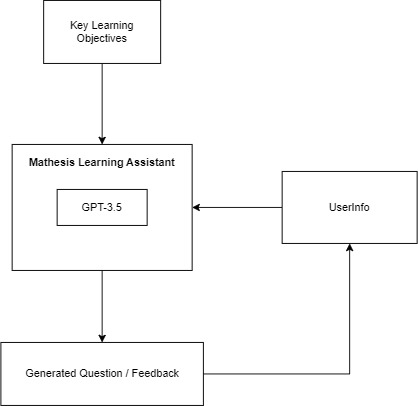
\includegraphics[width=0.8\textwidth]{Conceptual_diagram}
        \caption{Conceptual Model}
        \label{fig:conceptualModel}
    \end{figure}
    

    \paragraph{Mathesis}
    The core of our project is our \textit{Mathesis}
    learning assistant, powered by GPT 3.5.  This is placed at the center of the diagram, symbolizing
    its foundational role. It is important to include this component in our diagram as it is the main
    generator of content for the project.  This content can be anything from novel quiz questions to
    feedback for students. In our diagram, \textit{Mathesis} is shown as a wrapper with a core of
    GPT 3.5.  This is because our implementation is an extension and customization of GPT 3.5, created
    to achieve the project's specific goals. As the base model, GPT 3.5 provides the core language
    understanding and generation capabilities that the \textit{Mathesis} Learning Assistant will build
    upon.

    \paragraph{Key Learning Objectives}
    Also in our model, we include key learning objectives as an object.  This object represents the
    collection of core course material that students are meant to learn.  It is connected to our model,
    highlighting their guiding role in shaping the model's behavior through fine-tuning. These
    objectives ensure that the model focuses on the most important topics and concepts as defined by
    the faculty. The assistant generates questions and provides feedback on student's performance
    based on these key learning objectives.

    \paragraph{Model Output}
    In our diagram, we also include the products of the learning assistant.  This is important to include
    because it shows what the model actually does to deserve its role as central to the function of
    the project.  This output comes in the form of questions, generated from the learning objectives
    of the course, and useful feedback and corrections to the answers of students.  This feedback also
    encapsulates the char functionality of the model, where it provides feedback based on any question
    that the user asks of it.

    \paragraph{User Information System}
    Finally, the UserInfo MongoDB Database stores user information and their corresponding performance
    data for specific chapters.  This will be useful to help gauge the quality of the questions that
    the model produces and the areas that the students may be struggling the most in.  Both scenarios
    help to guide faculty into improving the course in some way.

    
    \subsection{Logical Model}
    
    Our logical model both maintains the objects and relations of the conceptual model and builds upon
    them through extra details about attributes any typing.

    \begin{figure}[h]
        \centering
        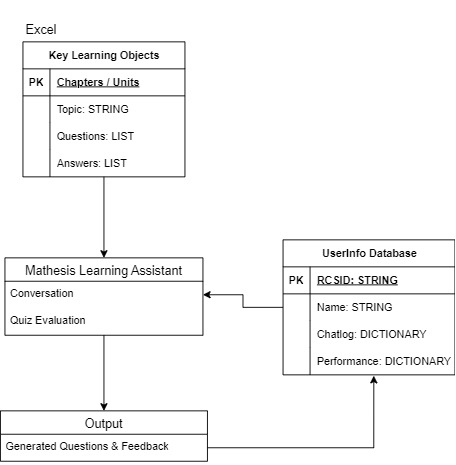
\includegraphics[width=0.8\textwidth]{Logical_diagram}
        \caption{Logical Model}
        \label{fig:logicalModel}
    \end{figure}

    \paragraph{Mathesis and Output}
    Our learning assistant comprises two main functionalities: Conversation and Quiz Evaluation.
    The model's conversational capabilities enable students to ask questions related to the learning
    topics, expanding their knowledge before formal evaluation. Quiz Evaluation is a functionality
    that grades chapter quizzes for students and records their performance. The 'Generated Questions
    \& Feedback' item in the Output object represents the quiz question generation process and the
    responses provided by the conversation functionality of the Mathesis Learning Assistant. 
    The 'Interface' object comprehensively represents the entire application, encompassing all its components and functionalities. 
    This includes the administrative view within the Mathesis Learning Assistant, which offers a specialized perspective tailored for administrators to have an overview of students' performance.

    \paragraph{Key Learning Objectives}
    For the faculty, the key learning
    objectives are stored in Excel sheets containing units, topics, questions, and answers that
    go into the internal representation that will guide our learning assistant.  Internally, this
    information is represented by a JSON file.  Within this file, we store each lesson, the core
    concepts that the lesson aims to teach, and any questions that \textit{Mathesis} generates based
    on those topics.

    \paragraph{User Information System}
    The UserInfo Database, with RCSID as the primary key, stores student information, including Name,
    Chatlog, and Performance.  This information is stored, ready to be put to use by the faculty.
    In the web interface, faculty have the ability to download a summary of student performance
    in either a csv or Excel format.



    \section{Prototype Implementation}

    Over the course of the project, we made several important decisions on how to best implement our
    prototype design.

    \subsection{Model Choice}

    One of the biggest references that we used in this decision-making process was
    the OpenAI Python API documentation~\cite{openAiDocs}.  This documentation details
    each of the models that we can use, their capabilities, and their drawbacks.  One example of this
    comes in the type of model that we use.  As our primary model, we use their \textit{text-davinci-003}
    model.  We have found that this model is a good balance between cost, quality, and flexibility.
    DaVinci is the most advanced of the \textit{text-*} models.  It offers similar quality to ChatGPT
    and has the added bonus of being available for file-tuning.  Using this feature helps to lower
    the uncertainty of our information system, as mentioned above.  An option that we did not decide to
    use as our primary model is \textit{gpt-3.5-turbo}.  This model is the model behind ChatGPT itself;
    it is more expensive and has the drawback of not being pre-trainable.  Due to these factors, we
    decided to keep using \textit{text-davinci-003} after the announcement of \textit{gpt-3.5-turbo}
    that came mid-way through the project.  This decision helps us to fulfil the first four of our
    \hyperref[functionalReqs]{functional requirements}.

    \subsection{Alternate Flows}

    Another important decision that we made was our decision to exclude particular alternative or
    error flows from our design.  From the beginning of this project, we have been aware that
    large language models, like the GPT series, can both be incredibly helpful and somewhat volatile.
    Notably, we considered the possibility that users could perform adversarial attacks on the model.
    While these attacks would only affect that particular student, it is important to make sure
    our model provides all students with an appropriate learning environment, regardless of their actions.
    This decision was influenced primarily by the \textit{DAN}~\cite{danThread} (Do Anything Now)
    exploit and its many iterations.  This exploit allows users to convince the ChatGPT model to
    ignore its alignment and safety training.  Attacks like these would likely also be able to
    bypass the fine-tuning of \textit{Mathesis}.  We have partially confirmed this assumption by
    testing similar exploits on GPT models.  We performed this evaluation by taking note of several
    topics that GPT disliked talking about and were able to convince the model to mention them.  For
    our experiment, we chose to focus on past political figures.  By speaking about adjacent topics
    then re-asking questions directed at these disallowed topics we were able to bypass the model's
    alignment somewhat.  Our evaluation suggests that students could attempt something
    similar if they wished to do so.  At present, we have decided to not work on measures
    specifically preventing this type of attack.  The reason for this is the relatively quick
    patches OpenAI sends out when exploits are discovered, combined with the difficulty of the
    problem.  Our hope is that this will not impact the functional requirements of the project,
    especially as OpenAI continues to work against the issue.

    \section{Conclusion}

    \subsection{Future Work}
    In our future work in this project, we expect to both finalize the attributes of the project that
    we have included in its current scope and to expand the projects scope to cover more edge cases.

    ...

    Ways in which we would expand the scope of the project would to be to better handle reasonable
    edge cases.  These could come in the form of students needing help with navigating the new system,
    handling adversarial attacks from students, or further automating the process of training models
    on new datasets.  These possible additions would serve to help students better adapt to using the
    \textit{Mathesis} assistant and its surrounding learning platform, deter students from using
    the model for unintended purposes, and creating encouraging environment for other professors who
    would like to include their courses into the learning system in future semesters respectively.

    \subsection{Closing Thoughts}
    ...

    \pagebreak
    
    \bibliographystyle{abbrv}
    \bibliography{references}
\end{document}
